\documentclass[12pt]{report}
\usepackage[utf8]{inputenc}
\usepackage{a4}
\usepackage[none]{hyphenat} %hyphenation
\sloppy
\usepackage{parskip} %no indentation after paragraphs
\usepackage{umlaute}
\usepackage{afterpage} %for using \afterpage{\clearpage} (don't push images to the end of a chapter)
\usepackage{makeidx}
\usepackage[numbers]{natbib}
\usepackage{picins} %provides precise control over the placement of inline graphics
\usepackage{setspace}
\usepackage{titlesec}
\usepackage{dsfont} %math symbols
\usepackage{tabularx}
\usepackage{floatflt} %float text around figures and tables
\usepackage{enumitem} %resume counting from previous enumerate block
\usepackage{amsmath,amssymb}
\usepackage[format=default,font=footnotesize,labelfont=bf]{caption}
\usepackage{listings} %for listing source code
\usepackage{color}
\usepackage{float} % for [H] after floats
\usepackage{url}
\usepackage{graphicx}
\usepackage{todonotes}
\usepackage[automake]{glossaries}
\newglossary[slg]{symbolslist}{syi}{syg}{Symbols}
\makeglossaries
\newacronym{CRDT}{CRDT}{Conflict-free replicated data type}
\newacronym{BFT}{BFT}{Byzantine Fault Tolerance}
\newacronym{PBFT}{PBFT}{Practical Byzantine Fault Tolerance}
\newacronym{PoW}{PoW}{Proof of work}
\newacronym{PoS}{PoS}{Proof of stake}
\newacronym{TPS}{TPS}{Transactions per second}
\newacronym{SDK}{SDK}{Software development kit}
 % all abbreviations
\newglossaryentry{symb:N}{sort={3},
name={$\mathbb N$},
first={first $\mathbb N$},
text={additional $\mathbb N$},
description={Set of natural numbers},
type=symbolslist} % all symbols
\glsaddall[types=\acronymtype]
\usepackage{listings}
\usepackage{color}
\definecolor{gray}{rgb}{0.4,0.4,0.4}
\definecolor{darkblue}{rgb}{0.0,0.0,0.6}
\definecolor{cyan}{rgb}{0.0,0.6,0.6}
\usepackage[autostyle]{csquotes}
\usepackage{subcaption}
\usepackage[ruled,lined,linesnumbered, noend]{algorithm2e}
\usepackage{algorithmicx}
\usepackage{algpseudocode}
\usepackage[]{algorithm2e}
\usepackage{multirow}
\usepackage{rotating}
\usepackage[toc,page]{appendix}
\usepackage{CJKutf8}
\usepackage{longtable}


\setlength{\extrarowheight}{10pt}

\lstset{
	basicstyle=\ttfamily,
	columns=fullflexible,
	showstringspaces=false,
	commentstyle=\color{gray}\upshape
}

\titleformat{\paragraph}[hang]{\normalfont\bfseries}{\theparagraph}{.5em}{}

\makeindex
\frenchspacing
\sloppy
\pagestyle{headings}
\textwidth16cm
\textheight22cm
\topmargin0cm
\oddsidemargin0cm
\evensidemargin0cm

\newcommand\tab[1][1cm]{\hspace*{#1}}

\newcommand{\bildklein}[4]{
	\begin{figure}[hp]
	\begin{center}
	\includegraphics[width=0.5\textwidth]{#1}
	\end{center}
	\caption[#2]{#3}
	\label{#4}
	\end{figure}
}
\newcommand{\bildgross}[4]{
	\begin{figure}[hp]
	\begin{center}
	\includegraphics[width=0.95\textwidth]{#1}
	\end{center}
	\caption[#2]{#3}
	\label{#4}
	\end{figure}
}

% This is tumlogo.tex
%
% Neues TUM-Logo in TeX
%   by G. Teege, 19.10.89
% Benutzung:
%   Am Anfang des Dokuments (TeX oder LaTeX):
%     \input tumlogo
%   Dann beliebig oft:
%     \TUM{<breite>}
%   bzw.
%     \oTUM{<breite>}
%   \TUM setzt das Logo mit der Breite <breite> und der entsprechenden Hoehe.
%   <breite> muss eine <dimen> sein. \oTUM erzeugt eine "outline"-Version
%   des Logos, d.h. weiss mit schwarzem Rand. Bei \TUM ist es ganz schwarz.
%   \oTUM entspricht damit der offiziellen Version des Logos.
%   Das Logo kann wie ein einzelnes Zeichen verwendet werden.
%   Beispiel:
%     Dies ist das TUM-Logo: \oTUM{1cm}.
%
\def\TUM#1{%
\dimen1=#1\dimen1=.1143\dimen1%
\dimen2=#1\dimen2=.419\dimen2%
\dimen3=#1\dimen3=.0857\dimen3%
\dimen4=\dimen1\advance\dimen4 by\dimen2%
\setbox0=\vbox{\hrule width\dimen3 height\dimen1 depth0pt\vskip\dimen2}%
\setbox1=\vbox{\hrule width\dimen1 height\dimen4 depth0pt}%
\setbox2=\vbox{\hrule width\dimen3 height\dimen1 depth0pt}%
\setbox3=\hbox{\copy0\copy1\copy0\copy1\box2\copy1\copy0\copy1\box0\box1}%
\leavevmode\vbox{\box3}}
%
\def\oTUM#1{%
\dimen1=#1\dimen1=.1143\dimen1%
\dimen2=#1\dimen2=.419\dimen2%
\dimen3=#1\dimen3=.0857\dimen3%
\dimen0=#1\dimen0=.018\dimen0%
\dimen4=\dimen1\advance\dimen4 by-\dimen0%
\setbox1=\vbox{\hrule width\dimen0 height\dimen4 depth0pt}%
\advance\dimen4 by\dimen2%
\setbox8=\vbox{\hrule width\dimen0 height\dimen4 depth0pt}%
\advance\dimen4 by-\dimen2\advance\dimen4 by-\dimen0%
\setbox4=\vbox{\hrule width\dimen4 height\dimen0 depth0pt}%
\advance\dimen4 by\dimen1\advance\dimen4 by\dimen3%
\setbox6=\vbox{\hrule width\dimen4 height\dimen0 depth0pt}%
\advance\dimen4 by\dimen3\advance\dimen4 by\dimen0%
\setbox9=\vbox{\hrule width\dimen4 height\dimen0 depth0pt}%
\advance\dimen4 by\dimen1%
\setbox7=\vbox{\hrule width\dimen4 height\dimen0 depth0pt}%
\dimen4=\dimen3%
\setbox5=\vbox{\hrule width\dimen4 height\dimen0 depth0pt}%
\advance\dimen4 by-\dimen0%
\setbox2=\vbox{\hrule width\dimen4 height\dimen0 depth0pt}%
\dimen4=\dimen2\advance\dimen4 by\dimen0%
\setbox3=\vbox{\hrule width\dimen0 height\dimen4 depth0pt}%
\setbox0=\vbox{\hbox{\box9\lower\dimen2\copy3\lower\dimen2\copy5%
\lower\dimen2\copy3\box7}\kern-\dimen2\nointerlineskip%
\hbox{\raise\dimen2\box1\raise\dimen2\box2\copy3\copy4\copy3%
\raise\dimen2\copy5\copy3\box6\copy3\raise\dimen2\copy5\copy3\copy4\copy3%
\raise\dimen2\box5\box3\box4\box8}}%
\leavevmode\box0}
% End of tumlogo.tex



\begin{document}

\hoffset=5mm
\thispagestyle{empty}
\begin{center}
	\bigskip \bigskip \bigskip
	\oTUM{6.0cm} \\
	\vspace*{0.8cm}
	{\huge \bf Technische Universität} \\
	\bigskip
	{\huge \bf München} \\
	\bigskip \bigskip \bigskip
	{\huge \bf Fakultät für Informatik} \\
	\bigskip \bigskip \bigskip
	{\Large \bf Master's Thesis in Informatik} \\
	\bigskip \bigskip \bigskip \bigskip \bigskip
	{\Large Hyperledger Fabric: Removing the Ordering Service} \\
	\bigskip \bigskip \bigskip \bigskip
	{\Large Levon Oganyan} \\
	\bigskip
	\begin{figure}[ht]
	\centering 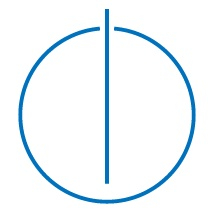
\includegraphics[width=0.2\linewidth]{figures/infologo.jpg}
	\end{figure}
	\bigskip
\end{center}
\vfill

\newpage
\hoffset=5mm
\thispagestyle{empty}
\begin{center}
	\bigskip \bigskip \bigskip
	\oTUM{6.0cm} \\
	\vspace*{0.8cm}
	{\huge \bf Technische Universität} \\
	\bigskip
	{\huge \bf München} \\
	\bigskip \bigskip \bigskip
	{\huge \bf Fakultät für Informatik} \\
	\bigskip \bigskip \bigskip
	{\Large \bf Master's Thesis in Informatik} \\
	\bigskip \bigskip \bigskip \bigskip \bigskip
	{\Large Hyperledger Fabric: Removing the Ordering Service} \\
	\bigskip \bigskip \bigskip
	{\Large Hyperledger Fabric: Die Entfernung des Bestellservices} \\
	\bigskip
\end{center}
\vfill
\begin{tabular}{ll}
{\Large \bf Author:} & {\Large Levon Oganyan} \\\\
{\Large \bf Supervisor:} & {\Large Prof. Dr. Hans-Arno Jacobsen} \\\\
{\Large \bf Advisor:} & {\Large Pezhman Nasirifard} \\\\
{\Large \bf Submission:} & {\Large xx.xx.20xx}
\end{tabular}

\newpage
\thispagestyle{empty}
\hoffset=0mm
\vspace*{\fill}
\noindent I confirm that this master's thesis is my own work and I have documented all sources and material used.\\\\
München, xx.xx.20xx\\\\\\\\\\\\
\noindent \textit{Levon Oganyan}

\newpage
\thispagestyle{empty}
\null

\newpage
\thispagestyle{empty}
\hoffset=0mm
\section*{Abstract}
\begin{spacing}{1.2}
Hyperledger Fabric provides a convenient framework for creating blockchain solutions. Like everything, it has room for improvement. One obvious improvement is the optimization of the ordering service. It is a bottleneck of the transaction flow and adds network delays which increase the chance of transactions becoming invalid. This thesis focuses on a specific scenario when transactions are conflict-free and commutative by design making the exact order of transactions not important. Under these circumstances the ordering service becomes redundant. Removal of the ordering service and the consequences of an orderless approach to Fabric is the topic of this thesis.

\end{spacing}

\newpage
\thispagestyle{empty}
\hoffset=0mm
\section*{Inhaltsangabe}
\begin{spacing}{1.2}
German Abstract
\end{spacing}

\newpage
\thispagestyle{empty}
\hoffset=0mm
\section*{Acknowledgment}
\begin{spacing}{1.2}
Acknowledgement 
\end{spacing}

\newpage
\setcounter{page}{1}
\hoffset=0mm
\fboxsep 0mm

\tableofcontents
\setcounter{tocdepth}{2}

\listoffigures
\addcontentsline{toc}{chapter}{List of Figures}

\listoftables
\addcontentsline{toc}{chapter}{List of Tables}

\printglossary[type=\acronymtype,style=long ,title=Abbreviations, toctitle=Abbreviations,nonumberlist]
\printglossary[type=symbolslist,style=long ,title=Symbols, nonumberlist]
\addcontentsline{toc}{chapter}{Abbreviations}

\newpage
\setlength{\baselineskip}{3ex}
\begin{spacing}{1.15}
\chapter{Introduction}
\label{chapter:introduction}

Since the creation and popularization of Bitcoin, numerous other blockchains were created. While some follow Bitcoin in its core ideas and implement the same type of consensus, namely Proof-of-work consensus, other blockchains employ different ways to reach consensus regarding the order of transactions. Bitcoin's choice of PoW is dictated by the permissionless nature of its network. PoW remains the sole practical way of reaching consensus in an open anonymous network where peers have zero trust towards each other. While providing means of reaching consensus Proof-of-work protocols have a low throughput measured in committed transactions per second. While this is not a problem in some scenarios, there are situations where high throughput is needed. If in these situations peers of the network have some degree of trust towards each other, an alternative solution can be used. Premissioned blockchains provide such a solution.

Hyperledger Fabric is an example of a permissioned blockchain. It provides a framework for creating high-throughput blockchains. However, there is always room for improvement. This thesis focuses on improving Hyperledger Fabric by optimizing its bottleneck, the ordering service under specific conditions.

\section{Motivation}
\label{sec:motivation}

Hyperledger Fabric employs a complicated network architecture. It's key part is the ordering service. Every transaction must eventually be sent to the orderer to be included in a block. Moreover, to avoid forks there can be only one ordering service in Fabric's network.

Also, since Fabric's transaction lifecycle separates the endorsement phase from the ordering or "adding to a block" phase and because of the extra network delays caused by this extra step, a lot of transactions become invalid by the time they reach the commit phase. These factors make the ordering service a natural bottleneck and a prime target for optimization.

\section{Problem Statement}
\label{sec:problemStatement}

The project targets a specific situation when the exact order of transactions is not relevant. For these cases, the best optimization is to remove the ordering phase altogether.

Even in the case when the order of transactions can be arbitrary, we would like to retain some properties of the original system.

\begin{itemize}
  \item Require endorsement of transactions according to a policy
  \item Keep a ledger of transactions
  \item Tamper-proof the ledger
\end{itemize}

The goal of the project is to create a premissioned blockchain based on Hyperledger Fabric that implements a transaction lifecycle without the ordering phase.

\section{Approach}
 \label{sec:approach}

\begin{itemize}
  \item Assume only conflict-free transactions.
  \item The world state is represented by a conflict-free replicated data type (CRDT).
  \item Keep the ordering service for configuration transactions and chaincode initialization.
  \item Keep the blockchain, pack transactions into blocks.
\end{itemize}

 Since there is no ordering system, there will be no consensus on the exact order of transactions. Nonetheless, this is not a problem, since CRDTs guarantee a consensus on the world state, provided that all transactions are committed to all peers. The approach is then to keep a separate, local blockchain on each peer node with it's own order.

 The new transaction lifecycle is as follows.
 The client sends transaction proposals to all endorsing peers as usual and collects endorsments. The endorsed transaction is then sent to all peers in the network. A peer receives the endorsed transaction, checks the signatures according to chain's policy and commits the transaction. After the transaction is committed, the peer send the client a receipt with the hash of the block the transaction was commited to. The client consideres the transaction as committed once it receives receipts from all peers.

\section{Organization} \label{sec:organization}
 The rest of the thesis is organized as follows. Chapter \ref{chapter:background} describes Hyperledger Fabric's network architecture and provides information about internal workings of the system. Chapter \ref{chapter:relatedWork} mentiones related work and precursors for this project.

 Chapters \ref{chapter:fabric} and \ref{chapter:sdks} detail the work done in this project. Chapter \ref{chapter:fabric} focuses on changes of Fabrics core systems and explains the new subsystem added by this project.
 Chapter \ref{chapter:sdks} describes changes in Hyperledger Fabrics SDKs and tools which enable users to access new features added to the Fabric.
 % \setlength{\parindent}{1em}
 % \indent Section \label{sec:app-approach} outlines the general implementation approach. Section  explains design decisions, problems and solutions of the initial implementation of the system.
 %
 % \indent Section  discusses subsequent improvements on the initial design.
 % \setlength{\parindent}{0pt}

 Chapter \ref{chapter:evaluation} describes the benchmark setup, benchmark chaincode and provides results of the testing. Chapter \ref{chapter:summary} discusses results of the project and outlines possible follow-up works.

\chapter{Background}
\label{chapter:background}

\section{Network}
\label{section:network}

In this section, we will dissect a basic network architecture. This example is based on the network used in chapter \ref{chapter:evaluation}. The section is based on \cite{fabricdocs:network}

For simplicity, the network has only one channel and two organizations.

\vskip 0.5cm

\begin{figure}[hp]
\begin{center}
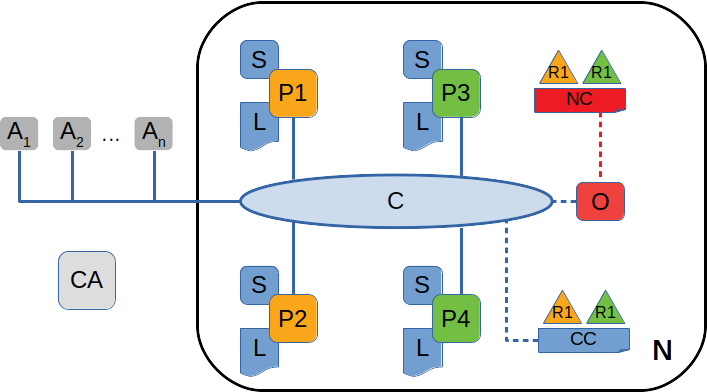
\includegraphics[width=0.95\textwidth]{figures/network}
\end{center}
\caption{Example of a Fabric network}
\label{fig:net}
\end{figure}

% \bildgross{figures/network}{}{Example of a Fabric network}{fig:net}

The network consists of two organizations $R1$ and $R2$. The network is under control of both R1 and R2 and is governed according to policy rules specified in the network configuration $NC$.

The network has four peers. Peers $P1$ and $P2$ belong to organization $R1$ and peers $P3$ and $P4$ belong to $R2$.

All four peers have joined a channel $C$ and maintain a copy of the channel's ledger $L$ and have a smart contract $S$ installed.

The channel is governed according to a channel policy, defined in channel configuration $CC$ and is controlled by both organizations.

An ordering service $O$ supports the channel and is ordering the channel's transactions into blocks and distributes blocks to the peers. It also serves as an administration point for the network. For administrative purposes, the ordering service uses a system channel, not shown in the diagram. The system channel is mandatory for any network and thus implicit.

Certificate authority $CA$ and applications $A_{1} ... A_{n}$ are not part of the network and in this specific case do not belong to a particular organization. In a general case

Applications are connected to the channel and can use its ledger and smart contract hosted on the peers to generate transactions and submit them to the ordering service. In this case, any application can use any peer to invoke the smart contract but in a general case, an application can only connect to peers from its organization.

Certificate authority issues and confirms certificates that are used to establish which applications or parts of the network belong to which organization. In this case, $CA$ is used by both organizations but in a general case, each organization can host its certificate authority server.

\newpage

\section{Transaction flow}
\label{section:flow}
This section describes a transaction flow or a transaction's lifecycle. The section is based on \cite{fabricdocs:flow},  \cite{fabricdocs:peer} and \cite{fabricdocs:orderer}

Fabric's transaction lifecycle consists of three phases
\begin{itemize}
  \item Proposal
  \item Ordering and packaging transactions into blocks
  \item Validation and commit
\end{itemize}

Let's say a client application wants to perform a transaction. It creates a transaction proposal and sends it to all peers whose signature is required, according to channels endorsement policy.
A peer receives the transaction proposal, checks that a client has necessary rights etc and executes it against the current ledger. The execution yields a read-write set. The set contains the keys which are read from and written to during the execution. The read part of the set also contains version value for each key. Versions are used later in the validation phase. The write part of the set contains keys and values that are to be written to commit the transaction to the ledger. The read-write set is then included in the response to the client and signed by the peer. The resulting structure is sent to the client. This concludes the Proposal phase.

When the client has collected all the required endorsements it checks them for consistency, packs them into a transaction envelope and sends the envelope to the ordering service. There can be different implementations of the ordering service, but they all perform the same function. The orderer receives transaction envelopes from different clients and assembles the incoming envelopes into blocks. After a  block is created, the order of transactions within it is fixed. The orderer then distributes the newly created block among the peers of the channel. This concludes the Ordering phase.

When a peer receives a block it goes through all transactions in the exact order they appear in the block. The peer checks signatures of a transaction and makes sure that it complies with the endorsement policy. Read-write sets from different endorsements are also checked for consistency. If a transaction passes all checks, the peer attempts to apply it to the ledger. Before applying a transaction, a ledger consistency check is done. The peer checks versions of the read keys to see if any of the keys were modified after the proposal was endorsed. If ledger state is compatible with the transaction, the transactions write set is applied and the transaction is marked as valid within the block. Invalid transactions are not applied but are marked as invalid and kept for accounting. The block is then appended to the chain and stored. Finally, the peer generates events, signaling to all subscribers which transactions were commited. This concludes the final phase of a transaction's lifecycle.

\section{The structure of a peer}

This segment describes some internal parts of a peer that are necessary for understanding the original work of this project.

A peer implements a number of services and consists of many subsystems. Endorser, Gossip, and KV-ledger subsystems are the relevant ones for the work.

\begin{figure}[hp]
\begin{center}
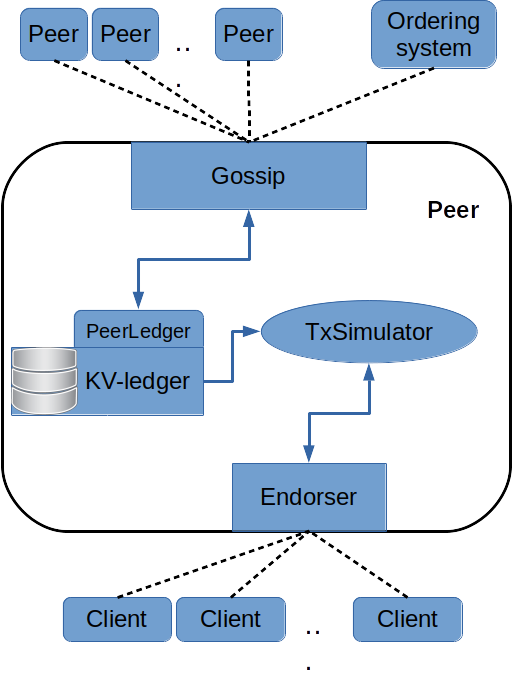
\includegraphics[width=0.5\textwidth]{figures/peer}
\end{center}
\caption{Relevant parts of a peer}
\label{fig:peer}
\end{figure}

Endorser subsystem is the one exposed to clients on the peer's side and it implements the Endorser gRPC service with a single call named ProcessProposal.
\begin{lstlisting}
rpc ProcessProposal(SignedProposal) returns (ProposalResponse) {}
\end{lstlisting}
SignedProposal is a structure sent by a client at the beginning of a transaction's lifecycle.

The Endorser subsystem executes the proposal, produces a read-write set as a result of the execution and creates a ProposalResponse which is used as an endorsement of the proposal by the client.  This subsystem has no direct access to the ledger. Access is provided indirectly through a transaction simulator (TxSimulator) produced by an endorser Support interface.

The Gossip subsystem handles all communications between all nodes of the network: peers and orderers alike. It is a big and intricate subsystem in and of itself and consists of many moving parts. However, for the purposes of the project, it is enough to know that Gossip handles block distribution and has capabilities to commit a block to the ledger.

KV-ledger subsystem implements PeerLedger interface and handles all the steps of committing a block to the ledger, described in \ref{section:flow}. It is at this stage when each transaction goes through MVCC validation when versions of keys from read set are compared with versions from the ledger for consistency

It is important to note, that the Gossip service is a singleton and it is possible to access it globally from any part of the peer. However, the Endorser does not access it in its code. On the contrary, there is an instance of KV-ledger subsystem for each ledger hosted on the peer and it's not accessible to write to from the Endorser.

\chapter{Related Work}
\label{chapter:relatedWork}

There is hardly any work directly related to the approach chosen by this project. Most of the optimizations of the ordering phase focus on improving the ordering service. There is no direct attempt at the removal of the ordering service as far as I was able to find out.

As mentioned in \ref{sec:app-noorder} one possible approach is to implement a peer-based PBFT consensus. Indeed there is a PBFT consensus in plans for Hyperledger Fabric, however, Fabric team's idea is to keep the ordering service logically and physically separate from peers. There will be a network of orderers that will receive endorsed transactions and decide on the ordering via a PBFT protocol. Resulting blocks will then be sent to the peers who have no say in the ordering decisions. At the moment Hyperledger Fabric is not Byzantine-fault tolerant and the new Raft ordering service is merely groundwork for a fully BFT ordering service as mentioned in \cite{fabricdocs:orderer}.

Another somewhat related work is \cite{lit:fabriccrdt} while it does not discuss the removal of the ordering service, it explores the application of CRDTs in Fabric. The idea is to use CRDTs to eliminate transaction conflict thus increasing the throughput of the network. However, transactions in \cite{lit:fabriccrdt} still go through the ordering service. This thesis is in a way a follow-up work. We use CRDTs to have non-conflicting order-less transactions and try to eliminate the ordering service as the next optimization.

\chapter{Approach}\label{chapter:approach}
Approach

\section{Approach}
Approach
\chapter{Evaluation}
\label{chapter:evaluation}

\section{Benchmark infrastructure}\label{sec:infra}

We use Caliper as a benchmark tool and HyperLedgerLab to set up the benchmark infrastructure and perform test runs. Modifications to these systems are described in \ref{sec:caliper} and \ref{sec:hll}.

The benchmark runs on an OpenStack cluster and consists of eight instances: three control nodes, three worker nodes, one load-balancer/DNS node, and one node for CLI. The CLI node is not used in the benchmark runs but is employed to set up the infrastructure and orchestrate the runs. Control and worker nodes are of the size m1.large. The rest is m1.medium.

{\color{red}Here will be \\technical details\\of m1.large \\and m1.medium \\once the cluster\\ is back online}

\newpage

\section{Benchmark chaincode}\label{sec:benchcode}

We use a simple chaincode with one core transaction to test the new Fabric. The ledger is initialized with one key: "VAR0" and a value 1. The transaction \textbf{moveVar} takes a new key as input, reads the value at "VAR0" and writes it to the new key. By itself,  \textbf{moveVar} is not conflict-free. This property is provided by the benchmark. For each transaction invocation, it picks a random key and invokes \textbf{moveVar} with that key as an argument. This, of course, does not guarantee the conflict-free property but makes transactions practically conflict-free.

\section{Testing plan}\label{sec:testplan}

First, we would like to see how changes in new parameters: batch size and batch timeout affect the throughput. Second, we would like to see if and how the number of peers and the number of organizations influence the throughput. In addition, we expect all or virtually all transactions to be committed. The testing plan is as follows:

\begin{table}[h!]
\begin{center}
\begin{tabular}{ c|c|c|c }
  \# Orgs & peers per org & batch size & batch timeout \\
 \hline
 \hline
 2 & 2 & 30 & 0.3 \\
 \hline
 2 & 2 & 50 & 0.2 \\
 \hline
 2 & 2 & 10 & 0.2 \\
 \hline
 2 & 3 & 50 & 0.2 \\
 \hline
 2 & 4 & 50 & 0.2 \\
 \hline
 3 & 1 & 50 & 0.2 \\
 \hline
 1 & 4 & 50 & 0.2 \\
 \hline
 1 & 3 & 50 & 0.2 \\
 \hline
 1 & 1 & 50 & 0.2 \\
 \hline
\end{tabular}
\end{center}
\caption{Benchmark networks}
\label{table:setups}
\end{table}

Each setup is tested under 100, 200 and 300 TPS with 10000 transactions each. Afterward, a single query transaction is submitted to check if peers respond with consistent results.

\section{Results}\label{sec:testres}

Raw numbers are presented in the Appendix \ref{apdx:1}. Here we present only the maximal throughput for each scenario and would like to discuss the results in general and what conclusions one can make from them.

\begin{table}[h!]
\begin{center}
\begin{tabular}{ c|c|c|c|c|c }
  \# Orgs & peers per org & batch size & batch timeout & throughput & avg latency, s \\
 \hline
 \hline
 2 & 2 & 30 & 0.3 & 242.5 & 11.02\\
 \hline
 2 & 2 & 50 & 0.2 & 252.4 & 7.97 \\
 \hline
 2 & 2 & 10 & 0.2 & 252.5 & 9.62 \\
 \hline
 2 & 3 & 50 & 0.2 & 213.8 & 16.94 \\
 \hline
 2 & 4 & 50 & 0.2 & 180.7 & 27.35 \\
 \hline
 3 & 1 & 50 & 0.2 & 247.7 & 10.52 \\
 \hline
 1 & 4 & 50 & 0.2 & 256.8 & 8.89 \\
 \hline
 1 & 3 & 50 & 0.2 & 280.3 & 3.52 \\
 \hline
 1 & 1 & 50 & 0.2 & 297.7 & 0.59 \\
 \hline
\end{tabular}
\end{center}
\caption{Benchmark results}
\label{table:results}
\end{table}

It turns out that under high load the batch size or the batch timeout changes show almost no effect on the throughput. The reason for that lies in the specifics of block processors implementation. Once enough transactions are collected, the block is issued and all clients receive a response, while the block is enqueued to be committed. The benchmark marks a transaction as committed when it receives a receipt, not when the actual block is committed. This approach might pose a problem in an industrial setting but is sufficient for a proof of concept.

Moreover, the number of organizations does not appear to affect throughput. The setup with 2 organizations with 2 peers in each organization, 4 in total, showed essentially the same throughput as the setup with 1 organization with 4 peers in it. This is to be expected since clients have to send the transaction envelope to all peers instead of sending it to one orderer and waiting for block events. It seems that the removal of the bottleneck of the ordering service might increase the throughput but severely hinder the scalability of the system.

However, the scalability issue might be ameliorated by employing anchor peers. Basically, make anchor peer of an organization keep a local ledger, and distribute the blocks of that ledger among the peers of its organization.

This approach has its own downsides. For example, it makes impossible endorsement policies that require endorsements from multiple peers of an organization.

Tests have not included the same variability of batch timeouts as with batch size since when testing under high load it becomes virtually irrelevant. When a peer receives more transactions per second than is enough to make a couple of batches, the batch size becomes the limiting factor of the throughput. However it seems to affect the average latency as does the block size.

\chapter{Summary} \label{chapter:summary}

Summary

\section{Status} 
\label{sec:status}

Final Status of the Thesis

\section{Conclusions}
\label{sec:conclusions}

Concluding remarks of Thesis

\section{Future Work} 
\label{sec:futureWork}

Future Work
\end{spacing}

\newpage
\begin{appendices}
\addtocontents{toc}{\protect\setcounter{tocdepth}{0}}
\chapter{Appendix}

\section{Results} \label{apdx:1}

\begin{table}[h!]
\begin{center}
\begin{tabular}{ |c|c|c|c|c|c|c|c|c| }
 \hline
  Test & Name & Succ  & Fail & Send TPS & Max lat, s & Min lat, s & Avg lat, s & Throughput \\
 \hline
 \hline
 1    & moveVar & 10000 & 0    & 99.1  & 1.10      & 0.02      & 0.22      & 98.8 \\
 \hline
 2    & moveVar & 10000 & 0    & 199.6 & 1.10      & 0.06      & 0.43      & 197.5 \\
 \hline
 3    & moveVar & 10000 & 0    & 263.0 & 34.44     & 0.21      & 11.02     & 242.5 \\
 \hline
 4    & getSum  & 4     & 0    & 58.0  & 21.02     & 20.94     & 20.98     & 0.2 \\
 \hline
\end{tabular}
\end{center}
\caption{2 Orgs, 2 peers per org, 30 batch size, 0.3s batch timeout}
\end{table}

\begin{table}[h!]
\begin{center}
\begin{tabular}{ |c|c|c|c|c|c|c|c|c| }
 \hline
  Test & Name & Succ  & Fail & Send TPS & Max lat, s & Min lat, s & Avg lat, s & Throughput \\
 \hline
 \hline
 1    & moveVar & 10000 & 0    & 99.3  & 1.39      & 0.03      & 0.37      & 99.1   \\
 \hline
 2    & moveVar & 10000 & 0    & 199.3 & 1.66      & 0.05      & 0.67      & 197.4  \\
 \hline
 3    & moveVar & 10000 & 0    & 273.7 & 26.14     & 0.38      & 7.97      & 252.4  \\
 \hline
 4    & getSum  & 4     & 0    & 108.1 & 21.25     & 21.00     & 21.13     & 0.2    \\
 \hline
\end{tabular}
\end{center}
\caption{2 Orgs, 2 peers per org, 50 batch size, 0.2s batch timeout}
\end{table}

\begin{table}[h!]
\begin{center}
\begin{tabular}{ |c|c|c|c|c|c|c|c|c| }
 \hline
  Test & Name & Succ  & Fail & Send TPS & Max lat, s & Min lat, s & Avg lat, s & Throughput \\
 \hline
 \hline
 1    & moveVar & 10000 & 0    & 99.8  & 0.70      & 0.02      & 0.16      & 99.7 \\
 \hline
 2    & moveVar & 10000 & 0    & 199.6 & 1.16      & 0.03      & 0.31      & 199.0 \\
 \hline
 3    & moveVar & 10000 & 0    & 294.1 & 33.05     & 0.07      & 9.62      & 252.5 \\
 \hline
 4    & getSum  & 4     & 0    & 53.3  & 9.11      & 9.03      & 9.05      & 0.4 \\
 \hline
\end{tabular}
\end{center}
\caption{2 Orgs, 2 peers per org, 10 batch size, 0.2s batch timeout}
\end{table}

\begin{table}[h!]
\begin{center}
\begin{tabular}{ |c|c|c|c|c|c|c|c|c| }
 \hline
  Test & Name & Succ  & Fail & Send TPS & Max lat, s & Min lat, s & Avg lat, s & Throughput \\
 \hline
 \hline
 1    & moveVar & 10000 & 0    & 99.6  & 1.25       & 0.03       & 0.36       & 99.3  \\
 \hline
 2    & moveVar & 10000 & 0    & 199.5 & 1.67       & 0.12       & 0.64       & 197.9 \\
 \hline
 3    & moveVar & 9996  & 4    & 249.4 & 41.48      & 0.49       & 16.94      & 213.8 \\
 \hline
 4    & getSum  & 4     & 0    & 20.9  & 27.25      & 18.27      & 24.88      & 0.1   \\
 \hline
\end{tabular}
\end{center}
\caption{2 Orgs, 3 peers per org, 50 batch size, 0.2s batch timeout}
\end{table}

\begin{table}[h!]
\begin{center}
\begin{tabular}{ |c|c|c|c|c|c|c|c|c| }
 \hline
  Test & Name & Succ  & Fail & Send TPS & Max lat, s & Min lat, s & Avg lat, s & Throughput \\
 \hline
 \hline
 1    & moveVar & 10000 & 0    & 99.2  & 1.66      & 0.07      & 0.66      & 98.7  \\
 \hline
 2    & moveVar & 10000 & 0    & 199.2 & 3.60      & 0.18      & 1.14      & 196.0 \\
 \hline
 3    & moveVar & 9927  & 73   & 260.9 & 52.37     & 0.49      & 27.35     & 180.7 \\
 \hline
 4    & getSum  & 0     & 4    & 25.2  & 0.00      & 100000.00 & NaN       & 0.0   \\
 \hline
\end{tabular}
\end{center}
\caption{2 Orgs, 4 peers per org, 50 batch size, 0.2s batch timeout}
\end{table}

\begin{table}[h!]
\begin{center}
\begin{tabular}{ |c|c|c|c|c|c|c|c|c| }
 \hline
  Test & Name & Succ  & Fail & Send TPS & Max lat, s & Min lat, s & Avg lat, s & Throughput \\
 \hline
 \hline
 1    & moveVar & 10000 & 0    & 98.8  & 1.29      & 0.02      & 0.31      & 98.6  \\
 \hline
 2    & moveVar & 10000 & 0    & 199.3 & 1.00      & 0.06      & 0.38      & 198.7 \\
 \hline
 3    & moveVar & 10000 & 0    & 285.8 & 32.79     & 0.37      & 10.52     & 247.7 \\
 \hline
 4    & getSum  & 4     & 0    & 56.3  & 10.55     & 10.48     & 10.52     & 0.4   \\
 \hline
\end{tabular}
\end{center}
\caption{3 Orgs, 1 peer per org, 50 batch size, 0.2s batch timeout}
\end{table}

\begin{table}[h!]
\begin{center}
\begin{tabular}{ |c|c|c|c|c|c|c|c|c| }
 \hline
  Test & Name & Succ  & Fail & Send TPS & Max lat, s & Min lat, s & Avg lat, s & Throughput \\
 \hline
 \hline
 1    & moveVar & 10000 & 0    & 99.4  & 1.20      & 0.03      & 0.30      & 99.4 \\
 \hline
 2    & moveVar & 10000 & 0    & 199.7 & 0.95      & 0.02      & 0.33      & 199.2 \\
 \hline
 3    & moveVar & 10000 & 0    & 286.0 & 28.11     & 0.09      & 8.89      & 256.8 \\
 \hline
 4    & getSum  & 4     & 0    & 26.1  & 23.18     & 7.31      & 19.15     & 0.2 \\
 \hline
\end{tabular}
\end{center}
\caption{1 Org, 4 peers per org, 50 batch size, 0.2s batch timeout}
\end{table}

\begin{table}[h!]
\begin{center}
\begin{tabular}{ |c|c|c|c|c|c|c|c|c| }
 \hline
  Test & Name & Succ  & Fail & Send TPS & Max lat, s & Min lat, s & Avg lat, s & Throughput \\
 \hline
 \hline
 1    & moveVar & 10000 & 0    & 99.4  & 1.14      & 0.02      & 0.30      & 99.4  \\
 \hline
 2    & moveVar & 10000 & 0    & 199.7 & 0.62      & 0.02      & 0.21      & 199.5 \\
 \hline
 3    & moveVar & 10000 & 0    & 296.6 & 13.69     & 0.07      & 3.52      & 280.3 \\
 \hline
 4    & getSum  & 4     & 0    & 81.6  & 10.25     & 9.86      & 10.13     & 0.4   \\
 \hline
\end{tabular}
\end{center}
\caption{1 Org, 3 peers per org, 50 batch size, 0.2s batch timeout}
\end{table}

\begin{table}[h!]
\begin{center}
\begin{tabular}{ |c|c|c|c|c|c|c|c|c| }
 \hline
  Test & Name & Succ  & Fail & Send TPS & Max lat, s & Min lat, s & Avg lat, s & Throughput \\
 \hline
 \hline
 1 & moveVar  & 10000  & 0 & 99.6 & 0.86 s & 0.02 s & 0.30 s & 99.5  \\
  \hline
 2 & moveVar  & 10000  & 0 & 199.7  & 0.68 s & 0.03 s & 0.29 s & 199.3 \\
  \hline
 3 & moveVar  & 10000  & 0 & 298.8  & 1.61 s & 0.10 s & 0.59 s & 297.7 \\
  \hline
 4 & getSum  & 4  & 0  & 190.5  & 10.55 s  & 10.52 s  & 10.53 s  & 0.4 \\
 \hline
\end{tabular}
\end{center}
\caption{1 Org, 1 peers per org, 50 batch size, 0.2s batch timeout}
\end{table}

\end{appendices}


\newpage
\bibliographystyle{ieeetr}
\bibliography{IEEEabrv,literature}
\end{document}
